\documentclass[12pt]{article}
\usepackage[utf8]{inputenc}
\usepackage{graphicx}
\usepackage{subcaption}
\usepackage{amsmath}
\usepackage{fancyhdr}
\usepackage{geometry}
\usepackage{dirtytalk}
\usepackage[english]{babel}
\usepackage{csquotes}
\usepackage{hyperref}
\usepackage{listings}
\usepackage{xcolor}
\usepackage{tikz}
\usetikzlibrary{shapes.geometric, arrows, positioning}

\lstset{
    language=C++,
    basicstyle=\ttfamily\small,
    numberstyle=\tiny,
    frame=single,
    breaklines=true,
    commentstyle=\color{green!50!black},
    keywordstyle=\color{blue},
    stringstyle=\color{red},
    showstringspaces=false,
    numbers=left
}

\linespread{1.25}
\setlength{\parindent}{0.8cm}
\setlength{\parskip}{0em}
\renewcommand{\headrulewidth}{0pt}
\geometry{a4paper, portrait, margin=1in}
\setlength{\headheight}{14.49998pt}
\graphicspath{{images/}}

% TikZ styles
\tikzstyle{startstop} = [rectangle, rounded corners, minimum width=3cm, minimum height=1cm, text centered, draw=black, fill=red!30]
\tikzstyle{process} = [rectangle, minimum width=3.2cm, minimum height=1cm, text centered, draw=black, fill=blue!20]
\tikzstyle{decision} = [diamond, minimum width=3.2cm, minimum height=1cm, text centered, draw=black, fill=green!20]
\tikzstyle{arrow} = [thick,->,>=stealth]
\tikzstyle{block} = [rectangle, draw, text width=7em, text centered, rounded corners, minimum height=3em]
\tikzset{every node/.style={align=center}}

\begin{document}
\begin{titlepage}
   \begin{center}
    \textsc{\large Ministry of Education of Republic of Moldova}\\[0.5cm]
    \textsc{\large Technical University of Moldova}\\[0.5cm]
    \textsc{\large Faculty of Computers, Informatics and Microelectronics}\\[0.5cm]
    \textsc{\large Software Engineering Department}\\[1.2cm]

    \vspace{25 mm}

    \textsc{\Large Embedded Systems}\\[0.5cm]
    \textsc{\large Laboratory work \#1.2}\\[0.5cm]

    \newcommand{\HRule}{\rule{\linewidth}{0.5mm}}
    \vspace{10 mm}
    \HRule \\[0.4cm]
    { \LARGE \bfseries User Interaction: STDIO - LCD + Keypad }\\[0.4cm]
    \HRule \\[1.5cm]

    \vspace{10mm}

    \begin{minipage}[t]{0.4\textwidth}
    \begin{flushleft} \large
    \emph{Author:} \\
    Sava \textsc{Luchian}\\
    std. gr. FAF-233
    \end{flushleft}
    \end{minipage}
    ~
    \begin{minipage}[t]{0.4\textwidth}
    \begin{flushright} \large
    \emph{Verified:} \\
    Alexei \textsc{Martiniuc}\\
    \end{flushright}
    \end{minipage}\\[3cm]

    \vspace{5 mm}
    \large Chisinau 2026\\[0.5cm]

    \vfill
    \end{center}
\end{titlepage}

\setcounter{page}{2}
\pagestyle{fancy}
\fancyhf{}
\rhead{\thepage}
\lhead{FAF-233 Sava Luchian; Laboratory Work No. 1.2}

\section*{Purpose of the Laboratory}
\hspace{0.8cm} To familiarize students with user interaction peripherals (LCD and 4x4 keypad) using STDIO services (\texttt{printf}, \texttt{fprintf}, \texttt{fscanf}) and implement an access-code verification application with visual feedback via LEDs.

\section*{Objectives}
\begin{enumerate}
    \item Understand basic principles of user interaction peripherals in embedded systems (LCD, keypad, LEDs)
    \item Use STDIO library for text exchange between user and MCU
    \item Design an MCU application that interprets keypad input and prints messages on LCD
    \item Develop a modular solution with separated peripheral and application modules
\end{enumerate}

\section*{Problem Definition}
\hspace{0.8cm} Configure the application for STDIO-based text exchange through LCD + keypad. Design an MCU application that detects a 4-digit code from a 4x4 keypad, validates it, and displays messages on LCD:
\begin{itemize}
    \item Valid code \textrightarrow~Green LED ON
    \item Invalid code \textrightarrow~Red LED ON
    \item Use STDIO for keypad scanning and LCD text printing
    \item Implement modular code architecture
\end{itemize}

\section{Domain Analysis}

\subsection{Technological Analysis and Application Context}
\hspace{0.8cm} The laboratory targets embedded Human-Machine Interaction (HMI) by combining a matrix keypad (user input), character LCD (user output), and status LEDs (binary visual feedback). The system is implemented on Arduino Uno (ATmega328P), chosen for deterministic timing, simple GPIO model, and compatibility with PlatformIO and Wokwi simulation.

STDIO is used as an abstraction layer over physical peripherals:
\begin{itemize}
    \item \texttt{printf()} for serial diagnostics
    \item \texttt{fprintf(lcdStream,...)} for LCD text output
    \item \texttt{fscanf(keypadStream,...)} for keypad character input
\end{itemize}

This approach provides a portable and structured I/O interface similar to classical C applications while preserving low-level hardware control.

\subsection{Hardware Components and Justification}
\begin{itemize}
    \item \textbf{Arduino Uno (ATmega328P)}: Main MCU at 16 MHz, 32 KB flash, 2 KB SRAM. Handles keypad scan events, LCD updates, and LED control.
    \item \textbf{LCD 16x2 (HD44780-compatible, 4-bit mode)}: Displays prompts, entered code, and result messages.
    \item \textbf{4x4 Matrix Keypad}: Captures user commands and 4-digit access codes.
    \item \textbf{Green LED + Red LED}: Shows success/failure state.
    \item \textbf{2x 220 $\Omega$ resistors}: Current limiting for LEDs.
    \item \textbf{Breadboard/Jumper wires/USB power}: Interconnection and 5V supply.
\end{itemize}

\subsection{Software Components}
\begin{itemize}
    \item \textbf{PlatformIO + VS Code}: Multi-file project support, dependency management, and reproducible builds.
    \item \textbf{Arduino Framework}: GPIO, timing, and serial abstractions.
    \item \textbf{Libraries}: \texttt{LiquidCrystal} and \texttt{Keypad}.
    \item \textbf{AVR-libc STDIO}: Stream setup with \texttt{fdev\_setup\_stream()}.
    \item \textbf{Wokwi Simulator}: Functional verification of the full hardware design.
\end{itemize}

\subsection{System Justification}
\hspace{0.8cm} The selected architecture separates peripherals from business logic, enabling reuse in subsequent labs. The design minimizes coupling by introducing a dedicated STDIO bridge layer, so application code does not directly depend on LCD/Keypad low-level APIs.

\section{Design}

\subsection{Architectural Sketch (HW--SW Integration)}

\begin{figure}[h!]
\centering
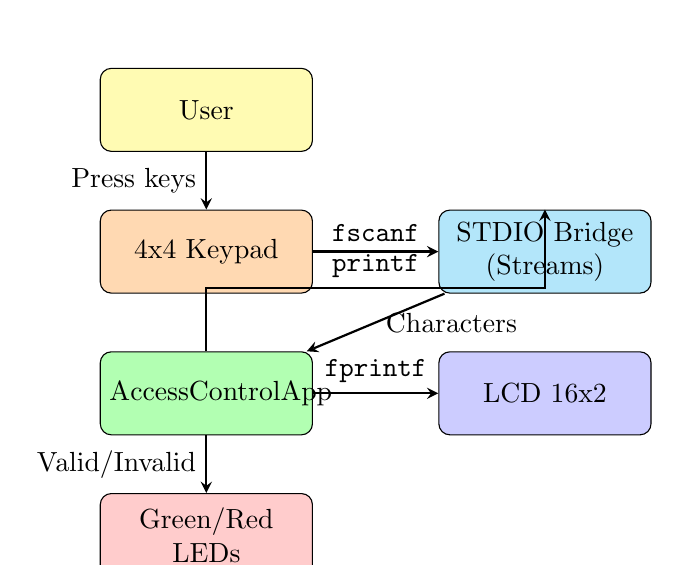
\begin{tikzpicture}[node distance=1.8cm]
    \node (user) [block, fill=yellow!30] {User};
    \node (keypad) [block, fill=orange!30, below of=user] {4x4 Keypad};
    \node (stdio) [block, fill=cyan!30, right of=keypad, xshift=2.5cm] {STDIO Bridge\\(Streams)};
    \node (app) [block, fill=green!30, below of=keypad] {AccessControlApp};
    \node (lcd) [block, fill=blue!20, right of=app, xshift=2.5cm] {LCD 16x2};
    \node (leds) [block, fill=red!20, below of=app] {Green/Red LEDs};

    \draw [arrow] (user) -- node[anchor=east]{Press keys} (keypad);
    \draw [arrow] (keypad) -- node[anchor=south]{\texttt{fscanf}} (stdio);
    \draw [arrow] (stdio) -- node[anchor=west]{Characters} (app);
    \draw [arrow] (app) -- node[anchor=south]{\texttt{fprintf}} (lcd);
    \draw [arrow] (app) -- node[anchor=east]{Valid/Invalid} (leds);
    \draw [arrow] (app.north) -- ++(0,0.8) -| node[anchor=south,pos=0.25]{\texttt{printf}} (stdio.north);
\end{tikzpicture}
\caption{Block architecture and software-hardware communication}
\label{fig:architecture}
\end{figure}

\textbf{Communication model:}
\begin{itemize}
    \item Input path: Keypad \textrightarrow~STDIO key stream \textrightarrow~application logic
    \item Output path: Application logic \textrightarrow~LCD STDIO stream and LED GPIO drivers
    \item Debug path: Application logic \textrightarrow~Serial monitor
\end{itemize}

\subsection{Electrical Sketch and Interconnection Explanation}

\textbf{Pin mapping used in implementation:}
\begin{itemize}
    \item LCD: RS=D13, E=D12, D4=D11, D5=D10, D6=D9, D7=D8, RW=GND, VO=GND, VCC=5V
    \item Keypad rows: D7, D6, D5, D4
    \item Keypad columns: D3, D2, A3, A2
    \item LEDs: Green=A0 (through 220 $\Omega$), Red=A1 (through 220 $\Omega$)
\end{itemize}

\begin{figure}[h!]
\centering
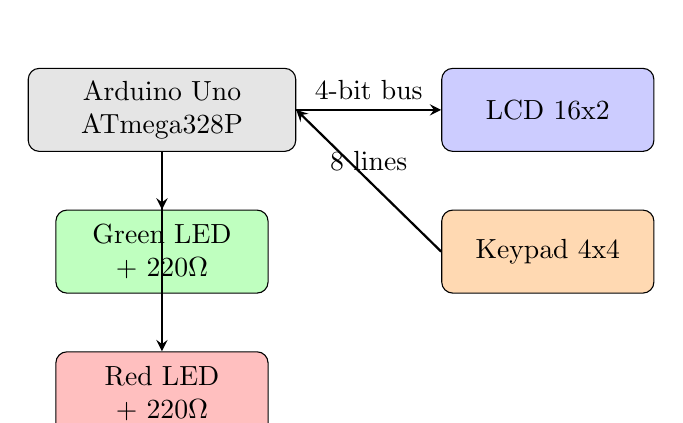
\begin{tikzpicture}[node distance=1.8cm]
    \node (uno) [block, fill=gray!20, text width=9em] {Arduino Uno\\ATmega328P};
    \node (lcd) [block, fill=blue!20, right of=uno, xshift=3.1cm] {LCD 16x2};
    \node (key) [block, fill=orange!30, below of=lcd] {Keypad 4x4};
    \node (gled) [block, fill=green!25, below of=uno] {Green LED + 220$\Omega$};
    \node (rled) [block, fill=red!25, below of=gled] {Red LED + 220$\Omega$};

    \draw [arrow] (uno) -- node[anchor=south]{4-bit bus} (lcd);
    \draw [arrow] (key.west) -- node[anchor=south]{8 lines} (uno.east);
    \draw [arrow] (uno) -- (gled);
    \draw [arrow] (uno) -- (rled);
\end{tikzpicture}
\caption{Electrical interconnection sketch (functional)}
\label{fig:electrical}
\end{figure}

\begin{figure}[htbp]
\centering
\includegraphics[width=0.9\textwidth]{schema.png}
\caption{Electrical circuit schema}
\label{fig:electrical-schema}
\end{figure}

\subsection{Behavioral Design (Finite-State Logic)}

\textbf{Main functional states:}
\begin{enumerate}
    \item \textbf{PROMPT}: Show \texttt{Enter Code:} and wait for first key
    \item \textbf{VERIFY}: Read 4 digits and validate against active code
    \item \textbf{RESULT}: Show \texttt{Access Granted} or \texttt{Access Denied}, set LEDs
    \item \textbf{CHANGE MODE (Optional)}: Triggered by key \texttt{A}; read old code, then new code
\end{enumerate}

\begin{figure}[h!]
\centering
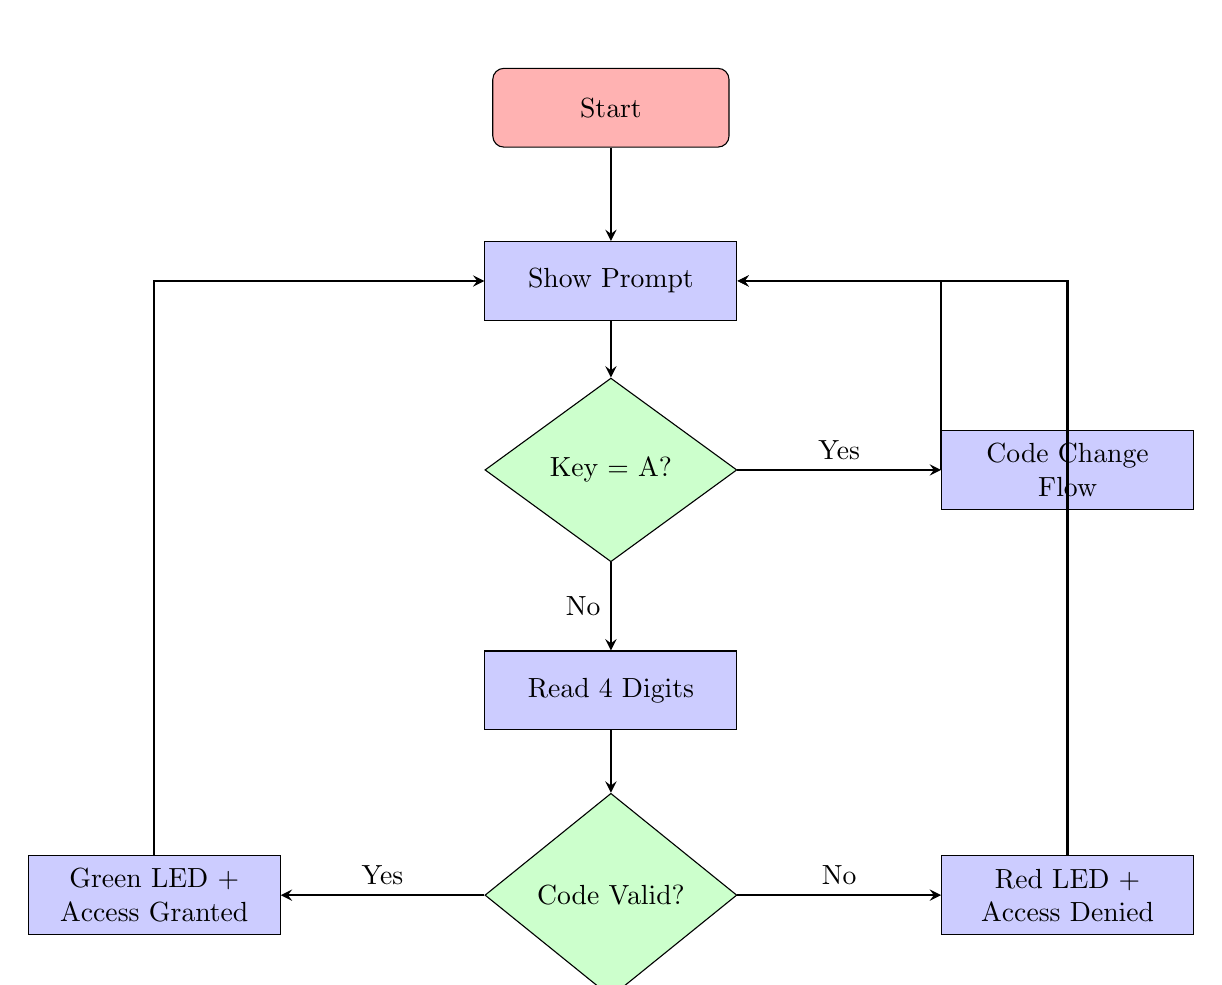
\begin{tikzpicture}[node distance=2.2cm]
    \node (start) [startstop] {Start};
    \node (prompt) [process, below of=start] {Show Prompt};
    \node (key) [decision, below of=prompt, yshift=-0.2cm] {Key = A?};
    \node (change) [process, right of=key, xshift=3.6cm] {Code Change\\Flow};
    \node (read) [process, below of=key, yshift=-0.6cm] {Read 4 Digits};
    \node (valid) [decision, below of=read, yshift=-0.4cm] {Code Valid?};
    \node (ok) [process, left of=valid, xshift=-3.6cm] {Green LED +\\Access Granted};
    \node (bad) [process, right of=valid, xshift=3.6cm] {Red LED +\\Access Denied};

    \draw [arrow] (start) -- (prompt);
    \draw [arrow] (prompt) -- (key);
    \draw [arrow] (key) -- node[anchor=south]{Yes} (change);
    \draw [arrow] (key) -- node[anchor=east]{No} (read);
    \draw [arrow] (read) -- (valid);
    \draw [arrow] (valid) -- node[anchor=south]{Yes} (ok);
    \draw [arrow] (valid) -- node[anchor=south]{No} (bad);
    \draw [arrow] (change.west) |- (prompt.east);
    \draw [arrow] (ok) |- (prompt.west);
    \draw [arrow] (bad) |- (prompt.east);
\end{tikzpicture}
\caption{Application flowchart}
\label{fig:flowchart}
\end{figure}

\subsection{Project Structure and Modular Implementation}

\begin{verbatim}
lab2/
|-- platformio.ini
|-- diagram.json
|-- wokwi.toml
|-- src/
|   |-- main.cpp
|   |-- config/
|   |   |-- AppConfig.h
|   |   `-- AppConfig.cpp
|   |-- peripherals/
|   |   |-- LedController.h/.cpp
|   |   |-- LcdDisplay.h/.cpp
|   |   `-- KeypadInput.h/.cpp
|   |-- io/
|   |   `-- StdioBridge.h/.cpp
|   `-- app/
|       `-- AccessControlApp.h/.cpp
`-- report/main.tex
\end{verbatim}

\textbf{Coding conventions and separation principles:}
\begin{itemize}
    \item Header/source separation for each module (interface vs implementation)
    \item CamelCase for classes and methods
    \item Magic numbers moved into \texttt{AppConfig}
    \item Single-responsibility modules for each peripheral/service
\end{itemize}

\section{Implementation}

\subsection{Description of Software Modules}
\begin{itemize}
    \item \textbf{AppConfig}: Constants for pins, keypad layout, code length, LCD dimensions.
    \item \textbf{LedController}: Controls green/red outputs (grant/deny feedback).
    \item \textbf{LcdDisplay}: Wraps LCD initialization and primitive display operations.
    \item \textbf{KeypadInput}: Wraps keypad scanning interface.
    \item \textbf{StdioBridge}: Implements stream redirection between STDIO and Serial/LCD/Keypad.
    \item \textbf{AccessControlApp}: Implements verification logic and optional code-change workflow.
\end{itemize}

\subsection{STDIO Utilization}
\hspace{0.8cm} The application uses STDIO in all critical paths:
\begin{itemize}
    \item \texttt{printf(...)} for serial diagnostics and interaction trace
    \item \texttt{fprintf(StdioBridge::lcdStream(), ...)} for LCD messages
    \item \texttt{fscanf(StdioBridge::keypadStream(), ...)} for keypad character acquisition
\end{itemize}

\textbf{Implementation concept:}
\begin{itemize}
    \item \texttt{fdev\_setup\_stream()} binds custom put/get functions to \texttt{FILE} streams.
    \item LCD stream handles cursor state and line transitions.
    \item Keypad stream blocks until a key is pressed, then returns one character.
\end{itemize}

\subsection{Functional Implementation Coverage}
\begin{enumerate}
    \item Read entered code from keypad (4 digits)
    \item Validate entered code against active code
    \item Display result on LCD
    \item Turn ON green LED for valid code
    \item Turn ON red LED for invalid code
    \item Optional feature: change code from keypad by pressing \texttt{A}
\end{enumerate}

\section{Results}

\subsection{Simulation and Build Evidence}
\textbf{Build result (PlatformIO):}
\begin{verbatim}
PLATFORM: Atmel AVR > Arduino Uno
Building .pio/build/uno/firmware.hex
[SUCCESS]
\end{verbatim}

\textbf{Wokwi runtime observations:}
\begin{itemize}
    \item Typing \texttt{1234} displays \texttt{Access Granted}; green LED turns ON
    \item Typing an incorrect code displays \texttt{Access Denied}; red LED turns ON
    \item Pressing \texttt{A} enters code-change mode (old code \textrightarrow~new code)
    \item After successful update, new code is accepted and old code is rejected
\end{itemize}

\begin{figure}[htbp]
\centering
\includegraphics[width=0.85\textwidth]{real_photo.jpg}
\caption{Real-life hardware assembly}
\label{fig:real-photo}
\end{figure}

\subsection{Representative Interaction Logs}
\begin{figure}[htbp]
\centering
\includegraphics[width=0.92\textwidth]{serial.png}
\caption{Serial terminal interaction log}
\label{fig:serial-log}
\end{figure}

\subsection{Performance and Resource Use}
\begin{itemize}
    \item Flash usage: ~9.4 KB (about 29\% of 32 KB)
    \item RAM usage: ~787 B (about 38\% of 2 KB)
    \item Response behavior: immediate user feedback suitable for educational HMI tasks
\end{itemize}

\section*{Note on AI Tool Usage}
\hspace{0.8cm} AI-assisted tools were used to support coding productivity and report drafting:
\begin{itemize}
    \item GitHub Copilot (code suggestions, refactoring support)
    \item LLM assistance for technical writing structure and language polishing
\end{itemize}
All generated content was manually reviewed, adapted, compiled, and validated against simulation behavior.

\section*{Bibliography}
\begin{enumerate}
    \item AVR-libc Documentation -- STDIO for AVR microcontrollers. \\
    \url{https://www.nongnu.org/avr-libc/user-manual/group__avr__stdio.html}

    \item Arduino Official Reference -- \texttt{Serial}, GPIO, and framework APIs. \\
    \url{https://www.arduino.cc/reference/en/}

    \item PlatformIO Documentation -- project configuration and toolchain. \\
    \url{https://docs.platformio.org/en/latest/}

    \item Keypad Library (Chris--A) -- matrix keypad handling for Arduino. \\
    \url{https://github.com/Chris--A/Keypad}

    \item LiquidCrystal Library -- HD44780 LCD control in 4-bit mode. \\
    \url{https://github.com/arduino-libraries/LiquidCrystal}
\end{enumerate}

\pagebreak

\section*{Annex -- Source Code and Artifacts}

\subsection*{Repository Artifacts}
\begin{verbatim}
lab2/
|-- platformio.ini
|-- diagram.json
|-- wokwi.toml
|-- README.md
|-- src/...
`-- report/main.tex
\end{verbatim}

\subsection*{Key Source Files}
\begin{itemize}
    \item \texttt{src/main.cpp}
    \item \texttt{src/app/AccessControlApp.h/.cpp}
    \item \texttt{src/io/StdioBridge.h/.cpp}
    \item \texttt{src/peripherals/LedController.h/.cpp}
    \item \texttt{src/peripherals/LcdDisplay.h/.cpp}
    \item \texttt{src/peripherals/KeypadInput.h/.cpp}
    \item \texttt{src/config/AppConfig.h/.cpp}
\end{itemize}

\subsection*{GitHub Repository}
\noindent\textbf{Repository URL:}\\
\url{https://github.com/Ekkusuu/embedded-systems-repo/tree/main/lab2}

\section{Conclusions}
\hspace{0.8cm} The laboratory objectives were met. A complete modular HMI solution was implemented on Arduino Uno using STDIO-mediated communication between keypad, LCD, and application logic. The final system validates 4-digit codes, provides clear visual status feedback through LEDs, and includes an optional runtime code-update feature.

Key outcomes:
\begin{enumerate}
    \item Practical integration of LCD + keypad with clean HW--SW boundaries
    \item Correct use of STDIO streams in an embedded context
    \item Reusable modular project structure for future laboratory work
\end{enumerate}

\end{document}
